\documentclass[12pt]{article}

%%%%%%%%%%%%%%%%%%%%%%%%%%%%%%%%%%%%%%%%%%%%%%%%%%%%%%%%%%%%%%%%%%%%%%%%%%%%%%%%
%                           Package preset for homework
%%%%%%%%%%%%%%%%%%%%%%%%%%%%%%%%%%%%%%%%%%%%%%%%%%%%%%%%%%%%%%%%%%%%%%%%%%%%%%%%
% Miscellaneous
\usepackage[margin=1in]{geometry}
\usepackage[utf8]{inputenc}
\usepackage{indentfirst}
\usepackage{blindtext}
\usepackage{graphicx}
\usepackage{xr-hyper}
\usepackage{hyperref}
\usepackage{enumitem}
\usepackage{color}
\usepackage{float}
% Math
\usepackage{latexsym}
\usepackage{amsfonts}
\usepackage{amssymb}
\usepackage{amsmath}
\usepackage{commath}
\usepackage{amsthm}
\usepackage{bbold}
\usepackage{bm}
% Physics
\usepackage{physics}
\usepackage{siunitx}
% Code typesetting
\usepackage{listings}
% Citation
\usepackage[authoryear]{natbib}
\usepackage{appendix}
\usepackage[capitalize]{cleveref}
% Title & name
\title{Homework}
\author{Tien Vo}
\date{\today}


%%%%%%%%%%%%%%%%%%%%%%%%%%%%%%%%%%%%%%%%%%%%%%%%%%%%%%%%%%%%%%%%%%%%%%%%%%%%%%%%
%                   User-defined commands and environments
%%%%%%%%%%%%%%%%%%%%%%%%%%%%%%%%%%%%%%%%%%%%%%%%%%%%%%%%%%%%%%%%%%%%%%%%%%%%%%%%
%%% Misc
\sisetup{load-configurations=abbreviations}
\newcommand{\due}[1]{\date{Due: #1}}
\newcommand{\hint}{\textit{Hint}}
\let\oldt\t
\renewcommand{\t}[1]{\text{#1}}

%%% Bold sets & abbrv
\newcommand{\N}{\mathbb{N}}
\newcommand{\Z}{\mathbb{Z}}
\newcommand{\R}{\mathbb{R}}
\newcommand{\Q}{\mathbb{Q}}
\let\oldP\P
\renewcommand{\P}{\mathbb{P}}
\newcommand{\LL}{\mathcal{L}}
\newcommand{\FF}{\mathcal{F}}
\newcommand{\HH}{\mathcal{H}}
\newcommand{\NN}{\mathcal{N}}
\newcommand{\ZZ}{\mathcal{Z}}
\newcommand{\RN}[1]{\textup{\uppercase\expandafter{\romannumeral#1}}}
\newcommand{\ua}{\uparrow}
\newcommand{\da}{\downarrow}

%%% Unit vectors
\newcommand{\xhat}{\vb{\hat{x}}}
\newcommand{\yhat}{\vb{\hat{y}}}
\newcommand{\zhat}{\vb{\hat{z}}}
\newcommand{\nhat}{\vb{\hat{n}}}
\newcommand{\rhat}{\vb{\hat{r}}}
\newcommand{\phihat}{\bm{\hat{\phi}}}
\newcommand{\thetahat}{\bm{\hat{\theta}}}

%%% Other math stuff
\providecommand{\units}[1]{\,\ensuremath{\mathrm{#1}}\xspace}
% Set new style for problem
\newtheoremstyle{problemstyle}  % <name>
        {10pt}                   % <space above>
        {10pt}                   % <space below>
        {\normalfont}           % <body font>
        {}                      % <indent amount}
        {\bfseries\itshape}     % <theorem head font>
        {\normalfont\bfseries:} % <punctuation after theorem head>
        {.5em}                  % <space after theorem head>
        {}                      % <theorem head spec (can be left empty, 
                                % meaning `normal')>

% Set problem environment
\theoremstyle{problemstyle}
\newtheorem{problemenv}{Problem}[section]
\newenvironment{problem}[1]{%
  \renewcommand\theproblemenv{#1}%
  \problemenv
}{\endproblemenv}
% Set lemma environment
\newenvironment{lemma}[2][Lemma]{\begin{trivlist}
\item[\hskip \labelsep {\bfseries #1}\hskip \labelsep {\bfseries #2.}]}{\end{trivlist}}
% Set solution environment
\newenvironment{solution}{
    \begin{proof}[Solution]$ $\par\nobreak\ignorespaces
}{\end{proof}}
\numberwithin{equation}{problemenv}

%%% Page format
\setlength{\parindent}{0.5cm}
\setlength{\oddsidemargin}{0in}
\setlength{\textwidth}{6.5in}
\setlength{\textheight}{8.8in}
\setlength{\topmargin}{0in}
\setlength{\headheight}{18pt}

%%% Code environments
\definecolor{dkgreen}{rgb}{0,0.6,0}
\definecolor{gray}{rgb}{0.5,0.5,0.5}
\definecolor{mauve}{rgb}{0.58,0,0.82}
\lstset{frame=tb,
  language=Python,
  aboveskip=3mm,
  belowskip=3mm,
  showstringspaces=false,
  columns=flexible,
  basicstyle={\small\ttfamily},
  numbers=none,
  numberstyle=\tiny\color{gray},
  keywordstyle=\color{blue},
  commentstyle=\color{dkgreen},
  stringstyle=\color{mauve},
  breaklines=true,
  breakatwhitespace=true,
  tabsize=4
}
\lstset{
  language=Mathematica,
  numbers=left,
  numberstyle=\tiny\color{gray},
  numbersep=5pt,
  breaklines=true,
  captionpos={t},
  frame={lines},
  rulecolor=\color{black},
  framerule=0.5pt,
  columns=flexible,
  tabsize=2
}


\title{Homework 1: Phys 7230 (Spring 2022)}
\due{January 24, 2022}

\begin{document}
\maketitle
%%%%%%%%%%%%%%%%%%%%%%%%%%%%%%%%%%%%%%%%%%%%%%%%%%%%%%%%%%%%%%%%%%%%%%%%%%%%%%%
\begin{problem}{1}
Consider two (otherwise) closed systems A and B at respective temperatures $T_A$
and $T_B$ in thermal contact with each other, so that heat $Q$ can flow between
them.

Using the 2nd law of thermodynamics -- total entropy $S$ of a closed system
increases under equilibration -- show that heat $Q$ flows from the hotter to the
colder system as $A$ and $B$ come to thermal equilibrium.

\textit{Hint}: $TdS\geq Q$.

\begin{solution}
First, assume $T_A>T_B$. Because these two systems are closed, the total energy
$U=U_A+U_B$ is constant. Thus $dU_B=-dU_A$. We need to prove that
$dU_A=Q<0$ (the hotter system loses heat $Q$ to the colder one as both systems 
come to equilibrium).

Now, the total entropy is $S=S_A+S_B$. Since the volume $V$ and number of
particles $N$ of each system are constant,
\begin{equation}
    dS=\qty(\frac{\partial S}{\partial U_A})_{N_A,V_A}dU_A
    +\qty(\frac{\partial S}{\partial U_B})dU_B
    =\qty(\frac1{T_A}-\frac1{T_B})dU_A\geq 0.
\end{equation}
The last inequality is the 2nd law of thermodynamics. Now, by assumption,
$1/T_A-1/T_B<0$, so it must be the case that $dU_A<0$ in order to make $dS\geq
0$. We are done.
\end{solution}
\end{problem}
\newpage
%%%%%%%%%%%%%%%%%%%%%%%%%%%%%%%%%%%%%%%%%%%%%%%%%%%%%%%%%%%%%%%%%%%%%%%%%%%%%%%
%%%%%%%%%%%%%%%%%%%%%%%%%%%%%%%%%%%%%%%%%%%%%%%%%%%%%%%%%%%%%%%%%%%%%%%%%%%%%%%
\begin{problem}{2}[Spin-1/2 paramagnet]
Consider a magnet of $N$ noninteracting spin-1/2 magnetic moments in an external
magnetic field $\vb{B}$, with Hamiltonian given by Zeeman energy,
\begin{equation}
    \HH=-\sum_{i=1}^N\bm\mu_i\vdot\vb{B}=-\sum_{i=1}^N\mu_BB\sigma_i
    \equiv-\sum_{i=1}^Nh\sigma_i
\end{equation}
where $\mu_B$ is Bohr magneton (carrying units of magnetic moment) and
$\sigma_i=\pm1$ labels the two Zeeman spin states of $n$th spin.

(a) For fixed dimensionless magnetization $M=N_\ua-N_\da$, (i) what is the
multiplicity $\Omega(M,N)$? (ii) What is the corresponding probability $P(M,N)$?
Check that $\sum_{M=-N}^NP(M,N)=1$.

(b) Compute the multiplicity $\Omega(E)$ for this system at a total energy $E$
and sketch/plot it as a function of full range of accessible energies. 

\textit{Hint}: Note that the magnetization $M$ is proportional to the energy
$E$.

(c) Derive the relation between temperature $T(E)$ and energy $E$ and plot
$T(E)$.

(d) Calculate the (i) magnetization $m(T,B)=\mu_B\sum_{i=1}^N\sigma_i$, (ii)
obtain its asymptotic forms in the classical $\mu_BB/k_BT\ll 1$ and quantum
$\mu_BB/k_BT\gg 1$ limits and (iii) plot it as a function of $T$ at a couple of
fixed values of $B$ and as a function of $B$ at a couple of fixed values of $T$.

\textit{Hint}: (i) Notice that magnetization is proportional to the energy $E$,
(ii) Eliminate $E$ in favor of $T$, (iii) Use lowest order Stirling
approximation throughout to simplify the factorials in your expression.

(e) Compute the linear magnetic susceptibility $\chi(T,B)=\eval{\partial
m/\partial B}_{B\to0}$, show that it exhibits Curie form
$\chi_\text{Curie}=a/T$, extracting the coefficient $a$.

(f) Compute the heat capacity (specific heat), $C_v(T)=T(\partial S/\partial
T)_{V,N}$, extract its low and high temperatures asymptotics, and sketch it,
noting its limiting forms and the crossover temperature.
\begin{solution}

(a) Given $M=N_\ua-N_\da$ and $N=N_\ua+N_\da$, we can write
\begin{equation}
    N_\ua=\frac{N+M}{2}\qquad\text{and}\qquad
    N_\da=\frac{N-M}{2}.
\end{equation}
(i) The multiplicity of $\Omega(M,N)$ is just the combination of $N_\ua$ in $N$
total paramagnets
\begin{equation}\label{p2a:Omega}
    \Omega(M,N)=\Omega(N_\ua,N_\da)
    =\binom{N}{N_\ua}
    =\frac{N!}{N_\ua!N_\da!}
    =\frac{N!}{\qty(\frac{N+M}{2})!\qty(\frac{N-M}{2})!}.
\end{equation}
(ii) For $N$ total paramagnets, each with 2 possible states, the sample size is
$2^N$. So the probability $P(M,N)$ is
\begin{equation}
    P(M,N)=\frac{\Omega(M,N)}{2^N}
    =2^{-N}\frac{N!}{\qty(\frac{N+M}{2})!\qty(\frac{N-M}{2})!}.
\end{equation}

Now, we check for the normalization condition of the probability $P$. Using the
binomial theorem:
\begin{equation}
    (1+1)^N=2^N=\sum_{N_\ua=0}^N\binom{N}{N_\ua}1^{N_\ua}1^{N-N_\ua}
    =\sum_{N_\ua=0}^N\Omega(N_\ua,N_\da).
\end{equation}
Converting the summation back to $M$, we get $-N\leq M\leq N$ for $0\leq
N_\ua\leq N$. Thus,
\begin{equation}
    1=2^{-N}\sum_{M=-N}^N\binom{N}{N_\ua}=\sum_{M=-N}^NP(M,N). 
\end{equation}

(b) By definition, $E=-hM$ with $h=\mu_BB$. So from \eqref{p2a:Omega},
\begin{equation}\label{p2b:Omega}
    \Omega(E)=\frac{N!}{\qty(\frac{N-E/\mu_BB}{2})!\qty(\frac{N+E/\mu_BB}{2})!}
\end{equation}
for $-\mu_BBN\leq E\leq\mu_BBN$. Figure\,\ref{fig:p2}(a) shows a plot of
\eqref{p2b:Omega}.

\begin{figure}[hbtp]
    \centering
    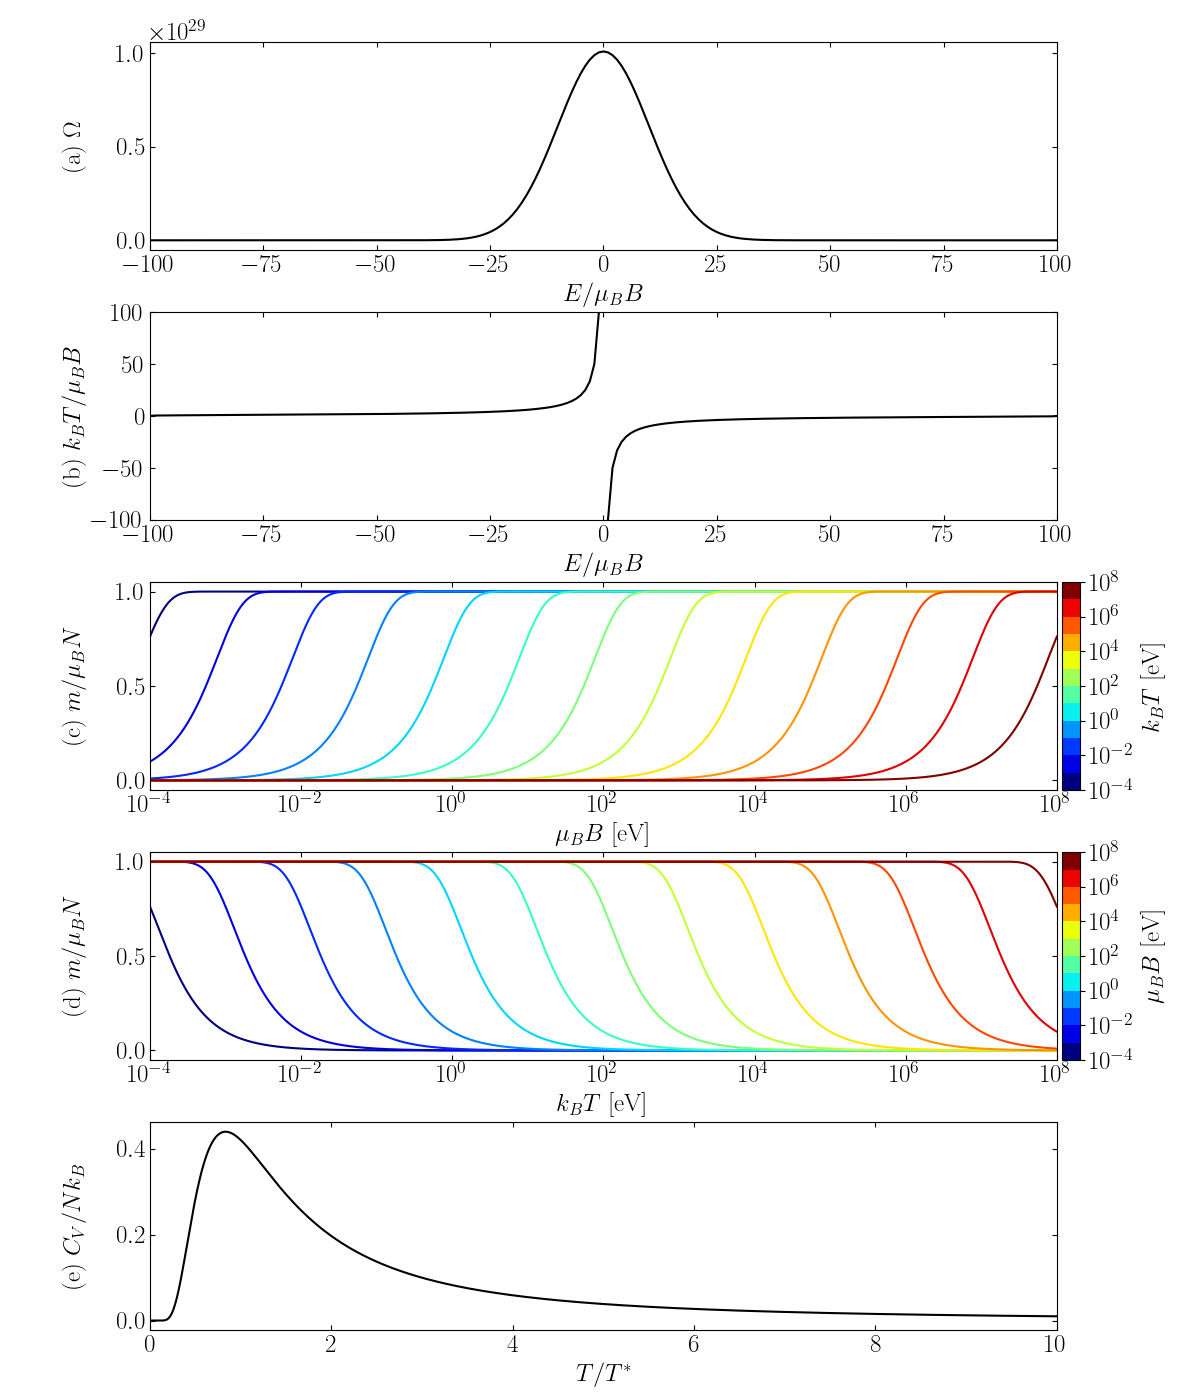
\includegraphics[width=\textwidth]{p2.png}
    \caption{Sketches of quantities in problem 2.}
    \label{fig:p2}
\end{figure}

(c) By definition, the entropy is
\begin{align}
    S/k_B
    &=\ln\Omega\notag\\
    &\approx N\ln N-N-\qty(\frac{N-E/\mu_BB}{2})\ln\qty(\frac{N-E/\mu_BB}{2})
    +\frac{N-E/\mu_BB}{2}\notag\\
    &\qquad-\qty(\frac{N+E/\mu_BB}{2})\ln\qty(\frac{N+E/\mu_BB}{2})
    +\frac{N+E/\mu_BB}{2}\notag\\
    &=N\ln N-\qty(\frac{N-E/\mu_BB}{2})\ln\qty(\frac{N-E/\mu_BB}{2})
    -\qty(\frac{N+E/\mu_BB}{2})\ln\qty(\frac{N+E/\mu_BB}{2})
\end{align}
by Stirling approximation. Using Mathematica to differentiate this wrt $E$, we
get
\begin{equation}
    \frac1{k_BT}=\frac{\partial(S/k_B)}{\partial E}=\frac1{2\mu_BB}
    \ln\qty(\frac{N-E/\mu_BB}{N+E/\mu_BB}).
\end{equation}
Thus, the temperature is
\begin{equation}\label{p2c:T}
    T=\frac{2\mu_BB}{k_B\ln\qty(\frac{N-E/\mu_BB}{N+E/\mu_BB})}.
\end{equation}
Figure~\ref{fig:p2}(b) shows the normalized temperature $k_BT/\mu_BB$.

(d) First, inverting \eqref{p2c:T}, we get
\begin{equation}
    E=-N\mu_BB\frac{e^{2\mu_BB}{k_BT}-1}{e^{2\mu_BB/k_BT}+1}
    =-N\mu_BB\tanh\qty(\frac{\mu_BB}{k_BT}).
\end{equation}
But the energy $E$ can also be written in terms of $m$ as $E=-mB$ since
$m=\mu_BM$. (i) So, the magnetization is
\begin{equation}\label{p2d:m}
    m=\mu_BN\tanh\qty(\frac{\mu_BB}{k_BT}).
\end{equation}
(ii) For $\mu_BB/k_BT\ll1$, $\tanh(x)\approx x$. Thus,
\begin{equation}
    m\qty(\frac{\mu_BB}{k_BT}\ll 1)=\frac{\mu_B^2NB}{k_BT}.
\end{equation}
For $\mu_BB/k_BT\gg 1$, $\tanh(x)\to1$, so the magnetization is a constant
\begin{equation}
    m\qty(\frac{\mu_BB}{k_BT}\gg1)=\mu_BN .
\end{equation}
(iii) Figure~\ref{fig:p2}(c-d) shows $m(T,B)/\mu_BN$ in various values.

(e) From \eqref{p2d:m}, we can calculate
\begin{equation}
    \chi=\lim_{B\to0}\frac{\partial m}{\partial B}
    =\frac{\mu_B^2N}{k_BT}\lim_{B\to0}\sech^2\qty(\frac{\mu_BB}{k_BT})
    =\frac{\mu_B^2N}{k_BT}.
\end{equation}
So $\chi$ follows Curie's law with the constant $a=\mu_B^2N/k_B$.

(f) By definition,
\begin{equation}
    C_v=T\frac{\partial S}{\partial T}
    =\frac{\partial E}{\partial T}
    =Nk_B\qty(\frac{\mu_BB}{k_BT})^2\sech^2\qty(\frac{\mu_BB}{k_BT}).
\end{equation}
For $x=\mu_BB/k_BT\ll 1$ (high temperature), $\sech(x)\to 1$ and the heat
capacity is
\begin{equation}
    C_v\qty(\frac{\mu_BB}{k_BT}\ll1)\approx Nk_B\qty(\frac{\mu_BB}{k_BT})^2.
\end{equation}
For $x\gg 1$ (low temperature), $\sech^2(x)$ dominates and so $C_v\to0$. Letting
the crossover temperature be $T^\ast=\mu_BB/k_B$, we can rewrite the heat
capacity in normalized form
\begin{equation}\label{p2f:Cv}
    \frac{C_v}{Nk_B}=\qty(\frac{T^\ast}{T})^2\sech^2\qty(\frac{T^\ast}{T}).
\end{equation}
Figure~\ref{fig:p2}(e) shows a plot of \eqref{p2f:Cv}.
\end{solution}
\end{problem}
\newpage
%%%%%%%%%%%%%%%%%%%%%%%%%%%%%%%%%%%%%%%%%%%%%%%%%%%%%%%%%%%%%%%%%%%%%%%%%%%%%%%
%%%%%%%%%%%%%%%%%%%%%%%%%%%%%%%%%%%%%%%%%%%%%%%%%%%%%%%%%%%%%%%%%%%%%%%%%%%%%%%
\begin{problem}{3}[Quamtum harmonic oscillators: Einstein solid]
Consider $N$ decoupled 3D quantum harmonic oscillators as a model of atomic
vibrations in a crystalline solid (Einstein phonons), described by the familiar
quantum Hamiltonian
\begin{equation}
    \hat\HH=\sum_{i}^N\qty[\frac{\hat{p}_i^2}{2m}+\frac12m\omega_0^2\hat{r}_i^2-\frac32\hbar\omega_0] 
\end{equation}
where for convenience I defined $\hat\HH$ with zero point energy subtracted off.

(a) Let's warm up on a single harmonic oscillator, computing its degeneracy
$g(n)=\Omega(E=\hbar\omega_0n)$ a fixed total energy
$E\equiv\hbar\omega_0n=\hbar\omega_0\sum_{\alpha=1}^dn_\alpha$ (where
$n_\alpha\in\Z$ are integer quantum numbers for $\alpha=x,y,\hdots$) for the
cases of (i) 2D and (ii) 3D.

(b) Recalling the eigenvalues
$E[\qty{n_\alpha}]=\hbar\omega_0\sum_{\alpha=1}^{3N}n_\alpha$
($\alpha=x_1,y_1,z_1,x_2,y_2,z_2,\hdots$ ranging from 1 to $3N$) for the
harmonic oscillator Hamiltonian, compute the multiplicity
\begin{equation}
    \Omega(E)=\sum_{\qty{n_\alpha}}\delta_{E,E[\qty{n_\alpha}]} 
\end{equation}
taking $E=\hbar\omega_0n$ ($n\in\Z$).

\textit{Hint}: Think about how to distribute $n$ total quanta of excitations
among $3N$ 1D oscillators, and use the lowest Stirling formula approximation for
$N\gg 1$ and $n\gg 1$.

(c) Compute the entropy $S(E)$ and the corresponding $T(E)$, thereby extracting
energy $E(T)$ as a function of temperature $T$, exploring its classical
$\hbar\omega_0/k_BT\ll1$ and quantum $\hbar\omega_0/k_BT\gg1$ limiting
functional forms. Plot $E(T)$, noting limiting forms.

(d) Compute heat capacity
$C_v=T(\partial S/\partial T)_{V,N}=\partial E/\partial T$ and explore its 
classical (high $T$) and quantum (low $T$) limits, showing
the expected equipartition $C_v=N_\text{dof}k_B$ in the former and its 
breakdown in the latter limits. Plot $C_v(T)$, noting the crossover temperature.

(e) Consider a classical limit of the problem with small $\hbar\omega_0/k_BT$
such that $E[\qty{n_\alpha}]=\sum_{\alpha=1}^{3N}\epsilon_\alpha$ and oscillator
eigenvalues $\epsilon_\alpha$ vary nearly continuously. Using this
simplification compute
\begin{equation}
    \Omega(E)=\Delta\prod_{\alpha=1}^{3N}\int\frac{d\epsilon_\alpha}{\hbar\omega_0}
    \delta(E-E[\qty{\epsilon_\alpha}]) 
\end{equation}
as a multidimensional integral over $\epsilon_\alpha$.

\textit{Hint}: It is helpful to use a result for a hypervolume of an
$N$-dimensional space spanned by positive values of $x_i$ coordinates, limited
by a hyperplane $x_1+x_2+\hdots+x_N=R$,
\begin{equation}
    V(R)=\int_{[\sum_{i=1}^Nx_i]\leq R}dx_1dx_2\hdots
    dx_N=\int_0^RdrS(r)=R^N/N!,
\end{equation}
where $S(R)=R^{N-1}/(N-1)!$ is the corresponding hyper-area at radius $R$ needed
for computation of the multiplicity $\Omega(E)$ and above integral is a
constrained one indicated by a prime.
\begin{solution}
(a) For the 2D case, there are two groups ($n_x,n_y$). The problem can be
understood in terms of a sequence of 0's (quanta) and 1's (partitions separting
groups). For example, if $n=5$, $000100$ is a possible sequence. Thus, there are
$n+1$ objects in total to shuffle and the (i) degeneracy is
\begin{equation}
    g_{2D}(n)=\binom{n+1}{n}=n+1.
\end{equation}
(ii) For the 3D case, there needs to be 2 partitions to separate the 0's into
three groups ($n_x,n_y,n_z$). So the degeneracy is
\begin{equation}
    g_{3D}(n)=\binom{n+2}{n}=\frac{(n+1)(n+2)}{2}.
\end{equation}

(b) Generalizing the previous results into the $3N$-dimensional case, there
needs to be $3N-1$ partitions to separate the 0's into $3N$ groups. The
multiplicity is thus
\begin{equation}
    \Omega=\binom{n+3N-1}{n}=\frac{(n+3N-1)!}{n!(3N-1)!}
    \approx\frac{(n+3N)!}{n!(3N)!}
\end{equation}
where we have assumed $n,N\gg 1$. Using the lowest order Stirling approximation
($N!\approx N^N$), we can simplify this result into
\begin{equation}
    \Omega(E)\approx\qty(1+\frac{3N\hbar\omega_0}{E})^{E/\hbar\omega_0}
    \qty(1+\frac{E}{3N\hbar\omega_0})^{3N}
\end{equation}
where we have also written $n=E/\hbar\omega_0$.

(c) By definition, the entropy is
\begin{align}
    S/k_B
    &=\ln\Omega\notag\\
    &=\frac{E}{\hbar\omega_0}\ln\qty(1+\frac{3N\hbar\omega_0}{E})
    +3N\ln\qty(1+\frac{E}{3N\hbar\omega_0})\notag\\
    &=3N\qty[\epsilon\ln\qty(1+\frac1\epsilon)+\ln\qty(1+\epsilon)]
\end{align}
where $\epsilon=E/3N\hbar\omega_0$. Differentiate wrt $E$,
\begin{equation}
    \frac{3N\hbar\omega_0}{k_BT}=\frac{\partial (S/k_B)}{\partial\epsilon}
    =3N\ln\qty(1+\frac1\epsilon)
\end{equation}
Thus, the temperature is
\begin{equation}
    T(E)=\frac{\hbar\omega_0}{k_B\ln\qty(1+3N\hbar\omega_0/E)} 
\end{equation}
Inverting this result, we get
\begin{equation}
    E(T)=\frac{3N\hbar\omega_0}{e^{\hbar\omega_0/k_BT}-1} 
\end{equation}

For the classical limit ($x=\hbar\omega_0/k_BT\ll 1$), $e^x-1\approx x$ and
$E(T)=3Nk_BT$. For the quantum limit ($x\gg1$), $e^x\to\infty$ and $E\sim
e^{-x}\to0$. The crossover temperature is $T^\ast=\hbar\omega_0/k_B$.
Figure~\ref{fig:p3c} shows that $E$ grows linearly at high temperature and
decreases to 0 in the quantum limit, as expected.
\begin{figure}[H]
    \centering
    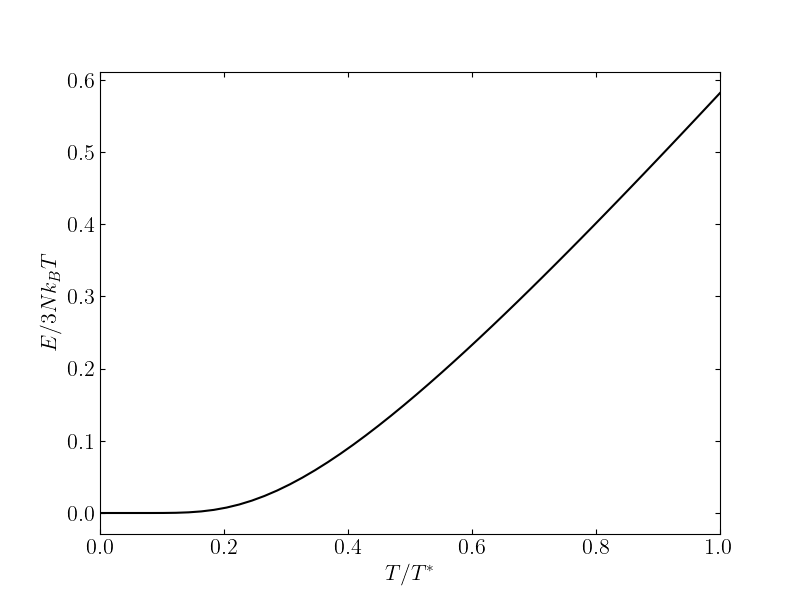
\includegraphics[width=0.6\textwidth]{p3c.png}
    \caption{$E(T)$ of $N$ decoupled 3D quantum harmonic oscillators.}
    \label{fig:p3c}
\end{figure}

(d) By definition,
\begin{equation}
    C_v=\frac{\partial E}{\partial T}
    =3Nk_B\qty(\frac{T^\ast}{T})^2\frac{e^{T^\ast/T}}{(e^{T^\ast/T}-1)^2}
\end{equation}
For the quantum limit, $C_v$ grows as $(T^\ast/T)^2e^{-T^\ast/T}\sim0$ because
of the exponential term. At large $T$ (classical limit), we can set $x=T^\ast/T$
and write $C_v$ as
\begin{equation}\label{p3d:C}
    C_v=3Nk_Bx^2\frac{e^x}{(e^x-1)^2}\approx3Nk_Bx^2\frac{1+x}{x^2}=3Nk_B 
\end{equation}
as $x\to0$. This is the expected equipartition where $N_\text{dof}=3N$.
Figure~\ref{fig:p3d} shows that the formal break occurs at $T=T^\ast$ as
expected. Also, $C_v$ is asymptotically constant as $T\to\infty$ as predicted in
\eqref{p3d:C} and decreases to 0 as $T\to0$.

\begin{figure}[H]
    \centering
    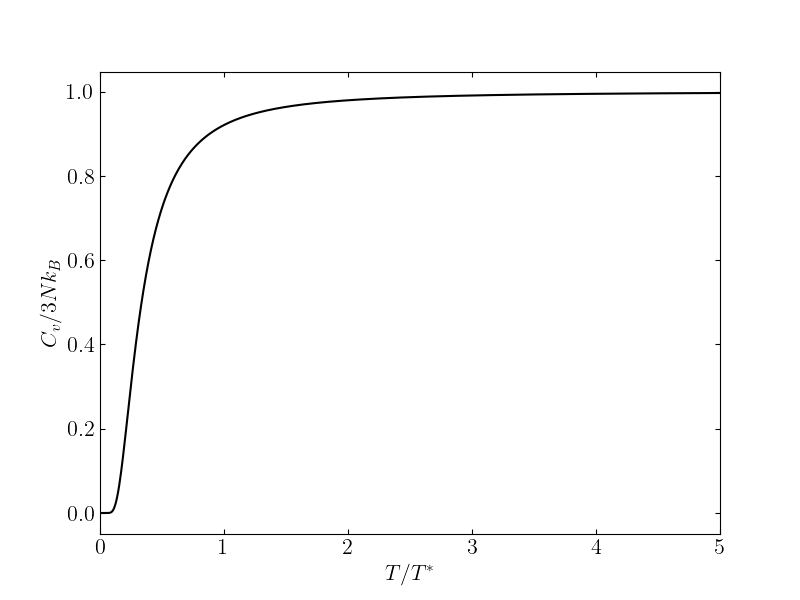
\includegraphics[width=0.6\textwidth]{p3d.png}
    \caption{$C_v(T)$ of $N$ decoupled 3D quantum harmonic oscillators.}
    \label{fig:p3d}
\end{figure}

(e) First, we can isolate the integration
\begin{equation}
    \Omega(E)=\frac{\Delta}{(\hbar\omega_0)^{3N}}
    \prod_{\alpha=1}^{3N}\int
    d\epsilon_\alpha\delta\qty(E-E[\qty{\epsilon_\alpha}])
    =\frac{\Delta}{(\hbar\omega_0)^{3N}}I_{3N}
\end{equation}

$I_{3N}$ is just the $(3N-1)$-dimensiona hyper-area restricted by the constraint
$E=\sum_{\beta=1}^{3N}\epsilon_\beta$ when integrating over a $3N$-dimensional
space $\R_+^{3N}$ where $R_+=[0,\infty)$. Thus,
\begin{equation}
     \Omega(E)=\frac{\Delta}{(\hbar\omega_0)^{3N}}S_{3N}(E)
     =\frac1{(3N-1)!}\frac{\Delta}{E}\qty(\frac{E}{\hbar\omega_0})^{3N}.
\end{equation}
But $(3N-1)!\approx (3N)!\approx (3N)^{3N}$ for $N\gg1$. So
\begin{equation}
    \Omega(E)\approx\frac{\Delta}{E}\qty(\frac{E}{3N\hbar\omega_0})^{3N} .
\end{equation}

\end{solution}
\end{problem}
\newpage
%%%%%%%%%%%%%%%%%%%%%%%%%%%%%%%%%%%%%%%%%%%%%%%%%%%%%%%%%%%%%%%%%%%%%%%%%%%%%%%
%%%%%%%%%%%%%%%%%%%%%%%%%%%%%%%%%%%%%%%%%%%%%%%%%%%%%%%%%%%%%%%%%%%%%%%%%%%%%%%
\begin{problem}{4}[Boltzmann gas]
Consider $N$ identical noninteracting particles in a 3D box of linear size $L$,
described by a Hamiltonian
\begin{equation}
    \HH(\qty{\vb{p}_i})=\sum_i^N\frac{p_i^2}{2m}
\end{equation}

(a) By integrating over $6N$ dimensional phase space, compute the multiplicity
(number of microstates) in a shell of width $\Delta$ around energy $E$,
\begin{equation}
    \Omega(E)=\frac{\Delta}{N!}\prod_{i}^N\qty[\int\frac{d\vb{r}_id\vb{p}_i}{(2\pi\hbar)^3}]\delta(E-\HH(\qty{\vb{p}_i})] 
\end{equation}
where $1/N!$ is the Gibbs ``fudge'' factor to crudely (we will see later why
this fix fails at low temperatures; also see below) account for the identity of
these classical particles, and we used the fact that 1 state corresponds to
phase space area $dxdp=2\pi\hbar$ to normalize the integration measure.

\textit{Hint}: Use the expression for a surface area of a $d$-dimensional unit
hypersphere, $S_d=2\pi^{d/2}/\Gamma(d/2)$ (with $S_2=2\pi,S_3=4\pi,\hdots$).

(b) Compute the corresponding (i) entropy $S(E,V,N)=k_B\ln\Omega$, and (ii) find
the temperature $T_c$ at which the entropy becomes negative, i.e., unphysical.

(c) Using the expression for $S(E,V,N)$ found above, calculate the pressure
$P(V,N)=T(\partial S/\partial V)_{E,N}$ for the Boltzmann gas, and show that it
leads to the familiar ideal gas law, $PV=Nk_BT$.

(d) Compute the corresponding chemical potential $\mu=-T(\partial S/\partial
N)_{E,V}$, expressing in terms of the thermal deBroglie wavelength
$\lambda_{dB}(T)=h/\sqrt{2\pi mk_BT}$, $T$ and density $n$.
\begin{solution}

(a) First, we can simplify
\begin{align}
    \Omega(E)
    &=\frac{\Delta}{E}\frac{V^N}{N!}\frac1{h^{3N}}\prod_i^N\int
    d\vb{p}_i\delta\qty(1-\sum_j^N\frac{p_j^2}{2mE})\notag\\
    &=\frac{\Delta}{E}\frac{V^N}{N!}\qty(\frac{2mE}{h^2})^{3N/2}\prod_i^N\int
    d\overline{\vb{p}}_i\delta\qty(1-\sum_j^N\overline{p}_j^2)\tag{$\overline{p}_j^2=p_j^2/2mE$}
\end{align}
The integration is now just the surface area of a $3N$-dimensional unit
hypersphere, since it is constrained to the surface
$1=\sum_j^N\overline{p}_j^2$. So we can write
\begin{align}
    \Omega(E)
    &=\frac{\Delta}{E}\frac{V^N}{N!}\qty(\frac{2mE}{h^2})^{3N/2}\frac{2\pi^{3N/2}}{\Gamma(3N/2)}\notag\\
    &\approx\frac{\Delta}{E}\frac{V^N}{\sqrt{2\pi N}e^{-N}N^N}\qty(\frac{2\pi
    mE}{h^2})^{3N/2}\frac{2}{\sqrt{3\pi N}e^{-3N/2}(3N/2)^{3N/2}}\notag\\
    &=\frac{2\Delta}{\sqrt6\pi NE}e^{5N/2}\frac{V^N}{N^N}\qty(\frac{4\pi
    mE}{3Nh^2})^{3N/2}
\end{align}
where we have written $\Gamma(3N/2)=(3N/2-1)!\approx(3N/2)!$ and used Stirling
approximation on the factorials.

(b) By definition, the (i) entropy is
\begin{equation}\label{p4b:S}
    S/k_B=\ln\Omega
    =\ln\qty(\frac{2\Delta}{\sqrt6\pi NE})+N\qty{\frac52
    +\ln\qty[\frac{V}{N}\qty(\frac{4\pi mE}{3Nh^2})^{3/2}]}
\end{equation}
the first term is small compared to $N$ and we retrieve the Sackur-Tetrode
equation in the last two terms. Also, the temperature (calculated with
Mathematica) is
\begin{equation}
    \frac1{k_BT}=\frac{\partial(S/k_B)}{\partial E}=\frac{3}2\frac{N}{E} 
    \Rightarrow\frac{E}{N}=\frac32k_BT
\end{equation}
Now, from \eqref{p4b:S}, $S<0$ only when
\begin{equation}
    \frac{V}{N}\qty(\frac{4\pi mE}{3Nh^2})^{3/2}
    =\frac{V}{N}\qty(\frac{2\pi mk_BT}{h^2})^{3/2}<e^{-5/2}
\end{equation}
(ii) Solving this inequality, we get
\begin{equation}
    T_c<\frac{h^2}{2\pi mk_B}\qty(\frac{N}{V})^{2/3}e^{-5/3}
\end{equation}

(c) Differentiating $S$ wrt $V$ (in Mathematica), we get
\begin{equation}
    \frac{P}{T}=\frac{\partial S}{\partial V}=\frac{Nk_B}{V} 
    \Rightarrow PV=Nk_BT
\end{equation}
This is the ideal gas law.

(d) Differentiating $S$ wrt $N$ (in Mathematica), we get
\begin{equation}
    \mu=-k_BT\ln\qty[\frac8{3\sqrt3}\frac{V}{N}\qty(\frac{\pi mE}{h^2N})^{3/2}]
    =-k_BT\ln\qty[\frac{1}{n}\qty(\frac{2\pi mk_BT}{h^2})^{3/2}]
    =k_BT\ln\qty(n\lambda_{dB}^3)
\end{equation}

\end{solution}
\end{problem}
\newpage
%%%%%%%%%%%%%%%%%%%%%%%%%%%%%%%%%%%%%%%%%%%%%%%%%%%%%%%%%%%%%%%%%%%%%%%%%%%%%%%
%%%%%%%%%%%%%%%%%%%%%%%%%%%%%%%%%%%%%%%%%%%%%%%%%%%%%%%%%%%%%%%%%%%%%%%%%%%%%%%
\begin{problem}{5}[Classical harmonic oscillators: Einstein solid]
Consider $N$ decouped 3D classical harmonic oscillators, described by the
familiar Hamiltonian
\begin{equation}
    \HH=\sum_i^N\qty[\frac{p_i^2}{2m}+\frac12m\omega_0^2r_i^2] 
\end{equation}
as the classical version of the problem above, with $\vb{r}_i,\vb{p}_i$ the
classical phase space coordinates. Let's repeat the analysis utilizing and
generalizing the analysis for the Boltzmann gas, above.

(a) By integrating over $6N$ dimensional phase space, compute the multiplicity
(number of microstates) in a shell of width $\Delta$ around energy $E$,
\begin{equation}
    \Omega(E,N)=\Delta\prod_i^N\qty[\int\frac{d\vb{r}_id\vb{p}_i}{(2\pi\hbar)^3}]\delta[E-\HH(\qty{\vb{p}_i})],
\end{equation}
where there is no $1/N!$ Gibbs ``fudge'' factor. Why?

(b) Compare your classical result with the high $T$ classical limit
($\hbar\omega_0/k_BT$ is the relevant dimensionless parameter) of the quantum
treatment of the system in problem 3(c,d,e) above.

(c) What is the relation of this classical analysis to the classical limit
analysis in problem 3e?
\begin{solution}

(a) 
\begin{align}
    \Omega(E,N)
    &=\Delta\prod_i^N\qty[\int\frac{d^3r_id^3p_i}{(2\pi\hbar)^3}]\delta(E-\HH(\qty{\vb{p}_i}))\notag\\
    &=\frac{\Delta}{E}\frac{1}{h^{3N}}
    \prod_i\int
    d^3r_id^3p_i\delta\qty[1-\sum_j^N\qty(\frac{p_j^2}{2mE}+\frac{m\omega_0^2r_j^2}{2E})]\notag\\
    &=\frac{\Delta}{E}\qty(\frac{4E^2}{(2\pi\hbar\omega_0)^2})^{3N/2}
    \prod_i^N\int
    d^3\overline{r}_id^3\overline{p}_i\delta\qty(1-\sum_j^N\overline{p}_j^2+\overline{r}_j^2)\tag{$\overline{r}_j^2=m\omega_0^2r_j^2/2E,\overline{p}_j^2=p_j^2/2mE$}\\
    &=\frac{\Delta}{E}\qty(\frac{4E^2}{(2\pi\hbar\omega_0)^2})^{3N/2}
    \frac{2\pi^{3N}}{\Gamma(3N)}\notag\\
    &\approx\frac{\Delta}{E}\qty(\frac{4E^2}{(2\pi\hbar\omega_0)^2})^{3N/2}\frac{2\pi^{3N}}{(3N)^{3N}}\notag\\
    &=\frac{\Delta}{E}\qty(\frac{E}{3N\hbar\omega_0})^{3N}
\end{align}
There is no fudge factor because the particles are distinguishable because of
the position in the Hamiltonian.

(b) From the previous results, the entropy is
\begin{equation}
    S=3Nk_B\ln\qty(\frac{E}{3N\hbar\omega_0}) 
\end{equation}
Then
\begin{equation}
    \frac1T=\frac{\partial S}{\partial E}
    =\frac{3Nk_B}{E}
\end{equation}
and the temperature is
\begin{equation}
    T=\frac{E}{3Nk_B}
\end{equation}
and the energy in terms of temperature is
\begin{equation}
    E=3Nk_BT 
\end{equation}
This agrees with the classical limit of problem 3(c). Similarly,
\begin{equation}
    C_v=\frac{\partial E}{\partial T}=3Nk_B 
\end{equation}
which is the asymptotic limit that we've seen in \eqref{p3d:C}. The multiplicity
in Problem 3(e) is the exact same result that we derived in part (a).

(c) We're integrating over the entire 6D phase space here, while in problem
3(e), we integrate over the energies of each macrostate.
\end{solution}
\end{problem}
%%%%%%%%%%%%%%%%%%%%%%%%%%%%%%%%%%%%%%%%%%%%%%%%%%%%%%%%%%%%%%%%%%%%%%%%%%%%%%%
    
\end{document}
